\section{Motivation}

Despite the increasing pervasiveness of mobile devices, as noted by \citet{socialTV}, there is a surprisingly limited number of options for mobile users to access live streaming television. Tablet computer in particular open up diverse and interesting interactivity questions -- could exploiting physical interaction hold viewers attention, even during adverts they may otherwise have ignored? Furthermore, could the disparity in the number of viewers per viewing device between traditional televisions and mobile devices be constructively exploited to provide granularly targeted adverts?

In this section, we will first introduce the customer of this project, \textit{Inqb8r}, and explain their interest in the area of TV streaming on tablet computers. We'll examine the functionality of tablet computers and question the benefits that the pervasiveness, mobility and interactivity of them provide. We will then consider how suitable current television formats would be for tablet computers, and following this, consider how this could open up opportunities for new methods of advertising by utilising interactivity and granular targeting. We will summarise by explaining how these insights could improve viewer attentiveness to adverts and the relative impacts on the advertisers and users of such a platform.

\subsection{Interest by Inqb8r}
	\label{sec:motivation_inqb8r}
	
	This project has been the result of a project proposal (Appendix~\ref{sec:inqb8r_proposal}) by \textit{Inqb8r}\footnote{Inqb8r's website -- \footurl{http://inqb8r.tv}} for a TV service targeted at tablet computers that would make use of complimentary services, such as interactive overlays and supplementary statistics. Inqb8r is a UK based business which provides a platform for content owners and advertisers to expose their products and services to university students.

	Inqb8r are responsible for the development of Project4\footnote{Project4's website -- \footurl{http://www.project4.tv}} (Figure~\ref{fig:project4}), a TV streaming service targeted towards students on Janet\footnote{Janet is a private network for education and research -- \footurl{https://www.ja.net/}}. Students are able to access the Project4 website in order to stream Channel~4, E4, More4, Film4 and 4Music, as well as it's own TV channel, studentTV. Project4 replace adverts broadcast by Channel~4 with adverts targeted specifically towards students.
	
	\begin{figure}[htb]
		\centering
			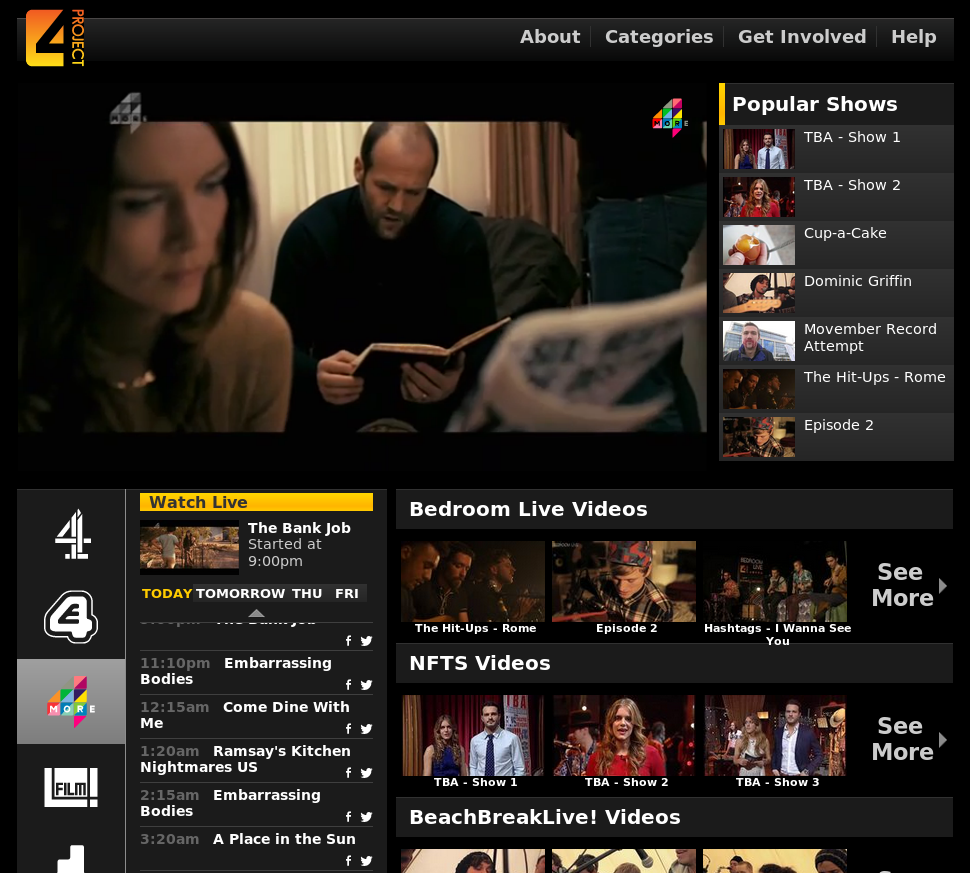
\includegraphics[width=0.5\textwidth]{images/project4.png}
		\caption{Project4 -- a student-oriented web-based TV service, which offers Channel~4 channels with adverts replaced with student-focused adverts.}
		\label{fig:project4}
	\end{figure}

	Inqb8r are interested in expanding the reach of Project4 by the creation of an application to watch TV on tablet computers. At present most of their users access the service via a web browser. This is in part due to their use of a Flash based player which is not compatible with many mobile devices, including iPads and other Apple devices. Modern technologies -- in particular, HTML5 -- allows video streaming in a web browser on these devices.

	Inqb8r expressed strong interest in researching how the touch displays and accelerometers of tablet computers may be used in providing interactive TV. One suggestion was to investigate the use of interactive overlays -- additional information displayed on top of a video stream, such as links to supplementary information, live polls and chats. They expressed interest in understanding how such overlays would affect how viewers watch TV.
	
	%utilisation of new HTML5 technologies to open up their service to a wider audience. Furthermore as their software utilises an interactive overlay for basic control they are interested to see how interaction centric platforms such as iPads can be leveraged to provide greater viewer interest. They are particularly keen to see if integrating traditional second screen technologies directly into the viewing medium has an impact on usability and enjoyability. 

\subsection{Pervasiveness of tablet computers}
	% Why would tablet computers be an interesting area to research?

	The popularity of tablet computers has been increasing rapidly. In 2012, \citet{pewResearch} showed that 25\% of Americans now own tablet devices and \citet{viacom} states that 15\% of full length television shows are now watched on tablet devices. Statistics collected by the TabLens service\footnote{\footurl{http://www.comscore.com/Products/Audience_Analytics/TabLens}} support this, showing that most tablet owners use their tablet to watch video\footnote{Comscore -- Majority of Tablet Users Watch Video on their Device, 1 in Every 4 Viewers Pay to Watch (June 2012) -- \footurl{http://www.comscore.com/Insights/Press_Releases/2012/6/Majority_of_Tablet_Users_Watch_Video_on_their_Device}}. Furthermore, statistics\footnote{International Data Corporation (IDC) Raises Tablet Forecast for 2012 and Beyond As iOS Picks Up Steam, Android Gains Traction, and Windows Finally Enters the Market -- \footurl{http://www.idc.com/getdoc.jsp?containerId=prUS23833612}} from IDC (see Figure~\ref{fig:tablet_market_share}) show that the Apple iPad holds the largest market segment and their predictions for 2016 suggest that Apple will maintain a strong majority if current trends do not change.

	\begin{figure}[htb]
		\centering
			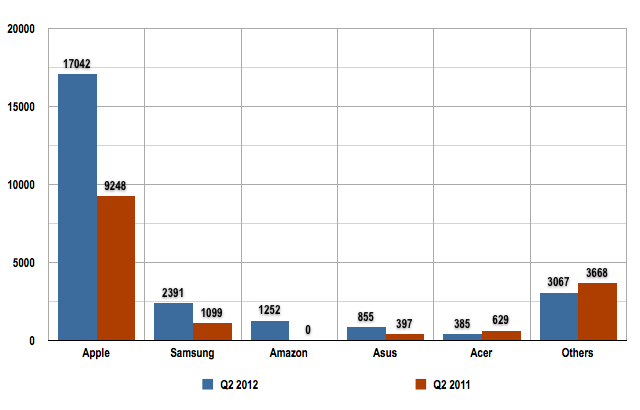
\includegraphics[width=0.6\textwidth]{images/idcTabletMarketShare.png}
		\caption[Caption for LOF]{Tablet Market Share (from reghardware.com\footnotemark, data source: IDC)}
		\label{fig:tablet_market_share}
	\end{figure}
	\footnotetext{Tablet market share -- \footurl{http://www.reghardware.com/2012/08/02/apple_leads_tablet_market_but_rival_shows_greater_growth/}}

	The mobility of tablet computers allows people to use applications from almost anywhere. [cite] demonstrates that using mobile devices occupy x\% of an average person's day, and describes that this may be due to their usage during commute times. This popularity and pervasiveness represents the demand for TV streaming on-the-go.

	Tablet computers offer large touch-screen displays, ideal for display video media and for providing interaction with media. 

	

\subsection{Evolution of television viewing}
	
	Since the invention of television, shows have been broadcast sequentially in the form of channels. The number of TV channels was restricted by the radio-wave frequencies that were available, however, digital broadcasting now allows more than one channel to be encoded into the same size of radio band \citep{DTVTransmission}. This has led to a dramatic increase in the number of channels available and has allowed broadcasters to expand their number of channels -- for example, Channel~4 (originally just one channel) now broadcasts six channels\footnote{Channel 4 Channels: Channel 4, E4, More4, 4Music, Film4, 4seven}. This allows the broadcaster to provide more content at any one time, an improve their reach by targeting multiple groups of people.

	However, the large choice of channels makes it difficult to search for a channel. TV listings are two-dimensional: an individual must search for a particular time under a particular channel in order to find a programme on at that time. This programme may be partly mitigated by Electronic Programme Guides (EPG) -- TV listings that are availabel electronically on digital TV recievers. An EPG may allow an individual to view what programmes are starting soon, reducing the channels they have to sift through. However, viewers are still limited to the choice of what is on now.

	Modern on-demand services, such as BBC iPlayer and 4oD, allow individuals to view what they want at any time. The choice of programmes may be huge, however, and may not be suitable for a user of a mobile device where searching is a problem due to... and may be frustrating

	The increased number of channels and range of methods of viewing TV has led to fragmentation of the TV-viewing market, as noted by \citet{audienceFragmentation} and \citet{informationOverload}. 
	
	[MORE!!!] and  both discuss the the rising issue of audience fragmentation. This is the reduction in the number of viewers per channel as more and more specialist channels emerge, attracting viewers to watch their tailored service in exclusion to all other channels. This helps somewhat with advertising, because if viewers are satisfied with the programmes and do not need to switch then the amount of valuable advertising time lost to transit becomes negligible as the user will learn the quickest way to navigate to their channel of choice. At the same time though this fragmentation also harms advertisers. Due to the migration of users to more focussed channels the number of users per channel decreases as the number of channels increases, meaning that advertisers need to pay for advert space on multiple channels to achieve the same reach, as most products will appeal to more than just the group watching one given show or focussed channel. This relative increase of advertising cost relative to effectiveness has also been noted by \citet{addressableAdvertisingOnDigitalTV} [ MORE!!!].

	%Furthermore, \citet{o2004improving} discusses
	EPG navigation by providing intelligent guides such as that in \citet{informationOverload}
	reducing the transit path such as in \citet{personalisedEPG}

	Traditionally users watch one show, on one channel and after show concludes each may switch to a different channel to watch another programme, stay on the same channel to watch the next show, or conclude their viewing session. This means adverts can be focussed towards the viewers likely to be watching a given show which is far easier than predicting the average viewership of an entire channel. However in-between two shows and when a user first turns on the television their attention is taken by the search for something to watch during which time they could have been watching shows or adverts if the search had not been there. They may also switch during a programme if it is boring them or there is a more preferred show starting on a different channel but this can still be considered the same type of interaction.

	When a show concludes or the user loses interest, it is typical for users to search for, then switch to a different channel. Searching for and navigating to their new desired channel, takes a significant amount of time also known as the transit time. During this time, adverts which the advertiser intended to be targeted to this viewer may be missed. This is because the advertisers assume that viewers watching before a show begins are watching to see that show and hence can target adverts towards those likely to enjoy the show. Therefore the large transit time inherent with a large number of channels reduces the amount of viewers who will see adverts targeted towards them. Even if the advertisers pay for an advert spot longer than the average transit time, having not seen the full advert, viewers who arrive late may not receive the full impact of the advert.

	If the requirement to search was lifted then this would provide a greater frequency (marketing term referring to the number of times a given viewer will see an advert) for a given value of investment. Research has shown that an OTS (Opportunities to see) value of 3 gives maximum ROI (return on investment) which is summarised by \citet{OTS} so maximising the number of viewers per spot means that to achieve an OTS of 3 an advertiser may need to pay for less actual spots to achieve the same number of viewers with an OTS of 3 allowing them to invest this money in other areas. Additionally a system which removes the tedious search, minimising the amount of non-viewing time in a given usage period, would likely be preferred by users over the current system and was predicted by \citet{cisco10Reasons}.



	While modern systems allow EPG data to be displayed and searched on the TV the fact that TV is live means that by the time a user has located a desirable show it may already have started. This is somewhat resolved by time-shifted channels which are simply rebroadcasts of other channels at a later time such as E4+1. Some services have also started offering 2 hour shifted channels but these still require a user to be present and ready at the exact time of broadcast. If users are more able to move to their next optimal channel, while minimising the transit time, this will mean they see a greater number of relevant adverts in a given usage period as they would be on a channel showing appealing content for a greater percentage of their time, hence if advertisers target their adverts to the shows well, then improving this situation could significantly improving the OTS values of relevant adverts.

	Having missed their show users then have two choices, hope that it will be rebroadcast on TV or use a TV catchup service such as 4oD. If the user chooses to use an on demand service then they likely have to sort through even more information as most catchup services provide at least the previous 7 days of content increasing the amount of time they must interact with the system before being able to watch their desired programme.

	Having considered these limitations and our resources, which included all the Channel 4 stream sources, we approached the issue of missing the start, or locating an engaging programme in a different way. We decided to provide the user with only one channel which would be generated when the user accesses our system by using what is known about them to build a playlist from all the live channels our system knows of, if there is nothing the user would find appealing on, or they have missed the start it will fall back to adding pre-recorded shows to the playlist until something appropriate started. As shows that have started are transparently skipped the user may miss a desired programme but because their channel consists of a mixture of live and recorded TV, once the show has been recorded it may be added to their playlist at a time when there is nothing engaging on live TV, meaning that users are able to watch without fear of missing shows at a time that suits them without the hassle usually involved in the process of locating a show.

\subsection{Beyond traditional advertising}
	Adverts generate revenue for the broadcaster and importantly are embedded in the stream at the source. This means that there is traditionally very little in the way of customisation. Advertisers pay for advert spots when they believe their target audience will be watching but it is unlikely that all of the viewers will be interested in the adverts. The user experience of any viewers who are not interested in the advert is negatively impacted in these situations. Some services such as YouTube have added the ability to skip their ads. This improves their overall user experience as if they find an advert annoying or offensive they have the ability to skip it. Furthermore other systems such as Facebook allow users to close adverts but request that the user says why they chose to close it. This provides useful feedback, helping to prevent inappropriate adverts and allowing advertisers to improve their future advertising campaigns.

	Unfortunately as the adverts are inserted at the source it is difficult to allow users of the TV medium to skip adverts when they are shown live. Although as user's may now record television they may simply watch it later and fast forward through the adverts meaning that it is more important than ever to maximize the viewer's enjoyment of adverts to reduce the likelihood of them using these functions.

	\subsubsection{Advert relevance and control}
		Despite the difficulty of skipping adverts systems such as Project4 do replace these adverts with more targeted ones through the use of triggered hardware. This is an important distinction because the hardware solutions are impractical for individual targeting as every user would need a separately ad-replaced stream. As much as users may desire it there is no way to skip an ad-break altogether. This is because the rest of the programme has not yet been broadcast so there is no media to return to. Therefore improving the user experience in current systems is limited to improving the relevance of adverts.

		We hypothesise that users would be more likely to enjoy an advert if it were relevant to them, with this assumption we can infer that personally recommended adverts targeted to each user would improve user interest, thus improving the user experience, whilst simultaneously providing advertisers with greater utility per impression, by maximising the likelihood that a viewer will be interested in their product. Additionally allowing the users to blacklist adverts should improve the user experience by allowing users to control which adverts they see and if they provide a reason for their disapproval, this is valuable feedback for advertisers to allow them to improve future adverts.

	\subsubsection{Interaction and engagement}
		We also hypothesise that if a user is less engaged by an advert then they may ignore it or even leave the room giving advertisers little or no utility and only annoying the users. Most current adverts do not take advantage of the interactive platform provided by tablet devices. There are second screen applications such as Shazam\footnote{Research Proves Shazam-Enabled TV Advertising Extends Engagement and Improves Effectiveness -- \footurl{http://www.businesswire.com/news/home/20121118005054/en/Research-Proves-Shazam-Enabled-TV-Advertising-Extends-Engagement}} which allow users to perform related tasks such as tagging the adverts which they see, which has been shown to increase brand recall but involves performing a supplementary task drawing attention from the advert. Providing the adverts interactively would reduce the requirements as only one device would be needed. This would also allow advertisers to provide useful or fun interactive content to reinforce the advert while still keeping partial attention on the original advert.

		By keeping the user focussed on the advert even if they do not pay direct attention to the content interaction provides another chance for users to remember the advert and provides greater benefit in advert repetition as users may interact with the advert even if they have seen the content before if it is entertaining or useful. For example in an advert for a film location data could be used to show the closest showings. When the user first sees the advert they may not be looking for a film, but later at the prompting of the advert they then have an instant interaction which may allow them to discover a showing at a local cinema starting soon thereby eliminating the search on a cinema's website reducing the length of the funnel required for a conversion.

\subsection{Individual targeting}
	\citep{socialTVPaper} argues that television is defined by the content that is viewed, not the device it is viewed on and that tablets are fast becoming one of the main devices people use to consume television. iPads and indeed most portable devices such as smart phones, tablets and laptops are typically used by a single person. Because of this many personal systems are already tightly integrated such as social media, like Twitter or Facebook. Additionally while a standard television may be watched by a whole family or more, anything watched on a tablet will likely be viewed by a single person, the owner. This means that adverts can be targeted individually to members of a family rather than trying to cover the full spectrum.

	Social interaction such as the action of liking something on Facebook can be easily integrated into adverts allowing users to save information on their personal profiles for later reference. This is useful in brand recall. For example if a user likes a brand that brand's Facebook posts will appear in their time-line reminding them of the brand and additionally providing a reference if they are having trouble recalling the product they saw advertised.

	\citep{socialTVPaper} further argues that television on the web are converging more and more to the point where the social experience has direct impact on what is broadcast as users can respond to what they see in the social sphere for example by Tweeting at a show or broadcaster. By extending the conclusions of \citep{socialTVPaper} we can infer that encouraging social participation in advertising would further allow users to control what they see and provide rich feedback to the advertisers which is confirmed by \citep{socialTV}.

	Systems such as ``Apple Airplay''\footnote{Technology to stream media to alternate devices -- \footurl{http://www.apple.com/airplay/}} can allow users to use their personal device as a source, and transmit media to a compatible endpoint device. This allows users to display something on their personal device on a more public device such as a television which can cause issues with individually targeted services.